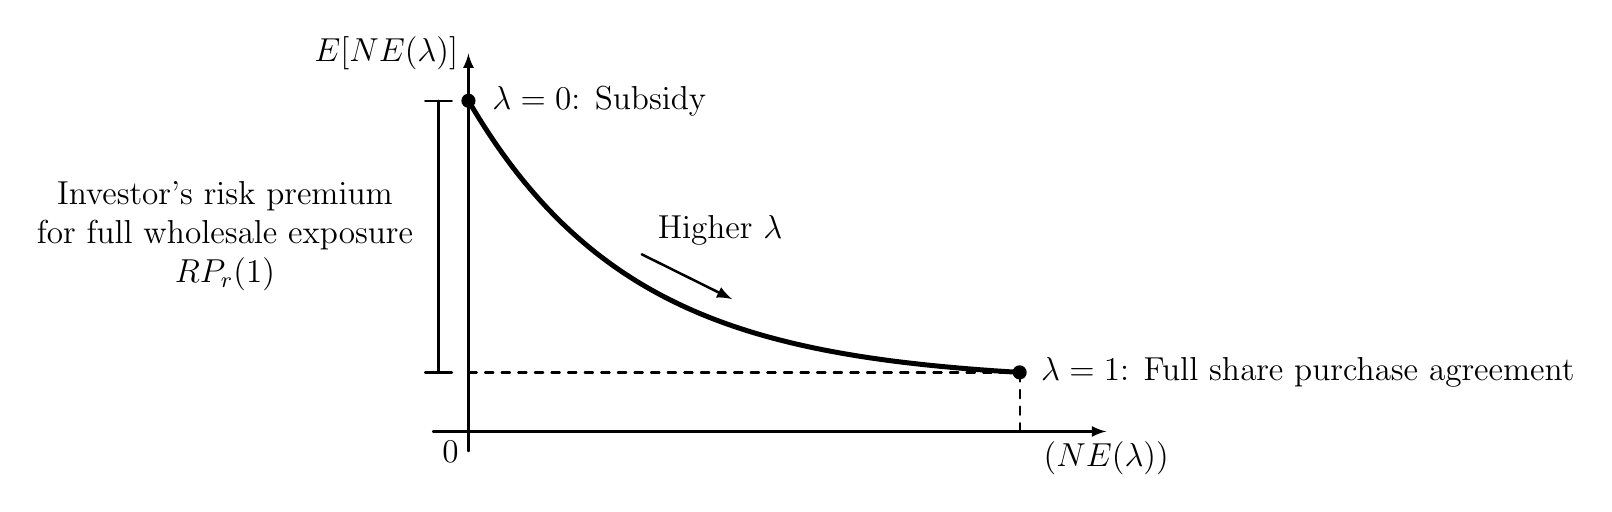
\begin{tikzpicture}[x=1cm,y=1cm,>=latex,line cap=round,line join=round]
  % Axes
  \draw[->, line width=0.8pt] (-0.45,0) -- (8.1,0)
    node[below,font=\large] {$\var(NE(\lambda))$};
  \draw[->, line width=0.8pt] (0,-0.25) -- (0,4.8)
    node[left,font=\large] {$E[NE(\lambda)]$};

  % Reference levels
  \draw[dashed, line width=0.8pt] (0,0.75) -- (7.0,0.75);
  \draw[dashed, line width=0.8pt] (7.0,0) -- (7.0,0.75);

  % Policymaker cost-risk frontier
  \draw[line width=1.8pt]
    plot[domain=0:7.0,samples=100]
    (\x,{0.75 + 3.45*(exp(-0.48*\x)-exp(-0.48*7))/(1-exp(-0.48*7))});

  % Endpoints
  \fill (0,4.20) circle (0.09);
  \fill (7.0,0.75) circle (0.09);

  % Risk-premium between the two endpoints
  \draw[line width=0.8pt] (-0.38,0.75) -- (-0.38,4.20);
  \draw[line width=0.8pt] (-0.55,0.75) -- (-0.21,0.75);
  \draw[line width=0.8pt] (-0.55,4.20) -- (-0.21,4.20);
  \node[align=center,left,font=\large] at (-0.58,2.48)
    {Investor's risk premium\\for full wholesale exposure\\$RP_r(1)$};

  % Labels
  \node[below left,font=\large] at (0,0) {$0$};
  \node[align=left,right,font=\large] at (0.18,4.20)
    {$\lambda=0$: Subsidy};
  \node[align=left,right,font=\large] at (7.15,0.75)
    {$\lambda=1$: Full share purchase agreement};

  \draw[->, line width=0.9pt] (2.2,2.25) -- (3.35,1.68);
  \node[above right,font=\large] at (2.28,2.25) {Higher $\lambda$};
\end{tikzpicture}
